\documentclass[a4paper,12pt]{ctexart}
\usepackage[style=gb7714-2015ay]{biblatex}
\usepackage{graphicx}
% \usepackage[scale=0.8]{geometry}
\usepackage{amsmath}
\usepackage{amssymb}
\usepackage{float}
\usepackage[hidelinks]{hyperref}

\providecommand{\keywords}[1]{\\\textbf{\textit{关键词:}} #1}
\addbibresource{reference.bib}
\title{绿色金融推动一带一路发展}
\author{董晨阳}
\date{\today}
\begin{document}
\maketitle
\begin{abstract}
    绿色必将成为推进共建“一带一路”高质量发展更加鲜明的底色。当前共建“一带一路”国家面临着排污权和发展权的矛盾,如何在发展的同时留下青山绿水对各国提出了挑战。绿色金融是缓和发展与环境之间矛盾的重要手段,本文通过整理共建一带一路国家的环境现状、估测绿色金融潜在的市场,并提出了一些政策建议。绿色金融在高质量共建“一带一路”方面大有可为。
\keywords{一带一路,绿色金融}
\end{abstract}
\clearpage
\section*{引言}

发展中国家往往面临污染权和发展权的权衡取舍\cite{曾文革2012从碳排放权之争看我国在气候变化上的法律应对}。大部分共建“一带一路”国家属于发展中国家,依赖高污染的行业可以使经济短期内粗放式快速发展,但代价却是牺牲环境、牺牲未来长期的发展利益。从自然资源禀赋及产业结构上看,很多“一带一路”国家能源结构相对依赖于传统化石能源,产业相对落后,经济社会发展、实现国家现代化的迫切愿望与追求绿色转型面临两难。如何运用政策和市场工具实现生态保护与经济发展的平衡,实现低排放、高增长的发展路径,对这些国家而言不仅是现实的挑战,也可能带来经济上的负担。
\begin{figure}[H]
    \centering
    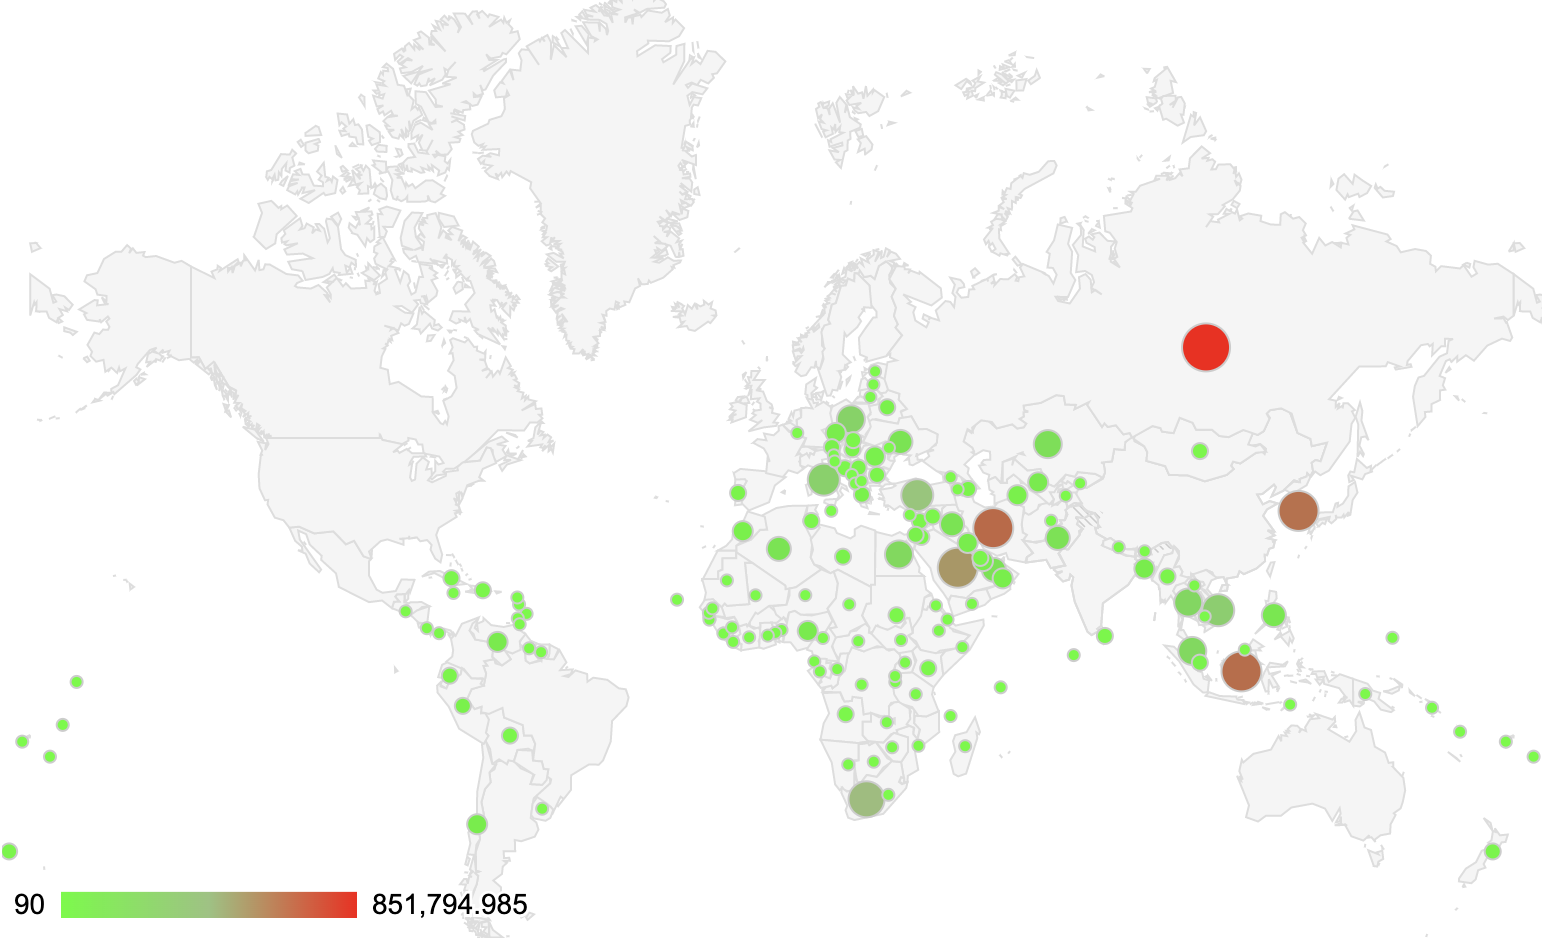
\includegraphics[width=0.8\linewidth]{./img/碳排放.png}
    \label{fig:carbonemit}
    \caption{一带一路国家2019年碳排放。数据来源:世界银行}
\end{figure}

绿色金融是缓解污染权和发展权矛盾的一种手段。绿色金融一种纳入环境因素的金融业务运作、产生环境效益的、服务于可持续发展的金融活动,例如为环境改善、气候变化和资源节约等领域开展投融资、项目运营、风险管理等金融服务,这些领域包括但不限于环保、节能、清洁能源、绿色交通、绿色建筑等领域。
绿色金融一方面意味着金融业要促进环境、经济、社会的可持续发展,能从资金端引导资金流向生态环境保护型产业,能从生产端引导企业生产注重绿色环保,从消费端引导消费者形成绿色消费理念;另一方面也意味着金融业自身的可持续发展,避免注重短期利益的过度投机行为。

通过绿色金融助力“一带一路”国家实现低碳转型具有紧迫性。
2019年,146个共建“一带一路”国家1碳排放总量约占全球30.8\%,显著高于其GDP占全球22.1\%的份额,且近5年增速远高于其它地区。同时,考虑到大部分“一带一路”国家仍处于工业化、城镇化的快速发展阶段,在未来一段时期内,碳排放规模仍将持续上升,可能成为新的“排放大户”。
\begin{figure}[H]
    \centering
    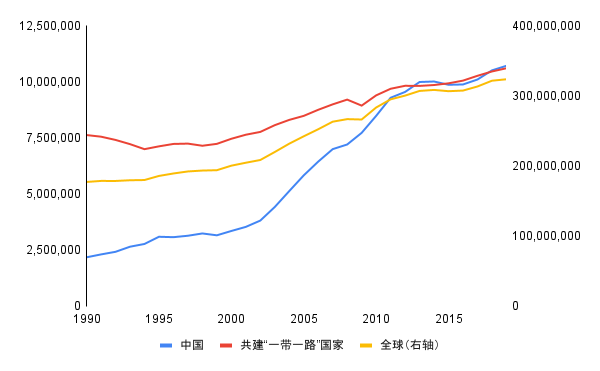
\includegraphics[width=0.8\linewidth]{./img/碳排放-折线图.png}
    \label{fig:carbonemit2}
    \caption{碳排放历史数据。数据来源:世界银行}
\end{figure}

通过绿色金融追求低碳发展也是共建“一带一路”国家的自身诉求。
作为全球应对气候变化的重要参与者,大部分“一带一路”国家积极支持和推动应对气候变化国际合作进程,参与多边框架谈判和国际规则制定,并在联合国气候变化框架公约下提交国家自主贡献承诺,在绿色能源、绿色建筑、绿色农业等领域提出相应的行动举措。
“一带一路”国家的生态环境相对脆弱、环境承载力不高,受全球气候变化影响和冲击可能更大,其率先实现绿色发展也更具紧迫性。

因此,通过绿色金融助力“一带一路”国家实现绿色转型具有充分的必要性和重要性。

\section*{文献综述}
\subsection*{何谓绿色金融}
关于绿色金融的定义,学界虽然没有统一的定义,但有一致的内涵,即联系起经济发展与环境保护,保持经济的可持续发展\cite{雷立钧2009绿色金融文献综述}。\citet{cowan1998topical}认为绿色金融是一种环境学和金融学的交叉学科,\citet{gray2002messiness}则认为是将社会与环境因素加入到金融学中,\citet{hohne2012mapping}认为绿色金融的内涵是随时间变化发展的,其定义取决于可持续性项目、环境政策等的定义。\citet*{张承惠2016发展中国绿色金融的逻辑与框架}则认为发达国家的定义偏重气候,由于他们已经完成了工业化,因而其认为即便是化石能源的更高效利用也不属于绿色金融;发展中国家则强调了发展属性,只要能够节约化石能源的使用量、降低单位能耗,相关投资都属于“绿色”
\begin{figure}[H]
    \centering
    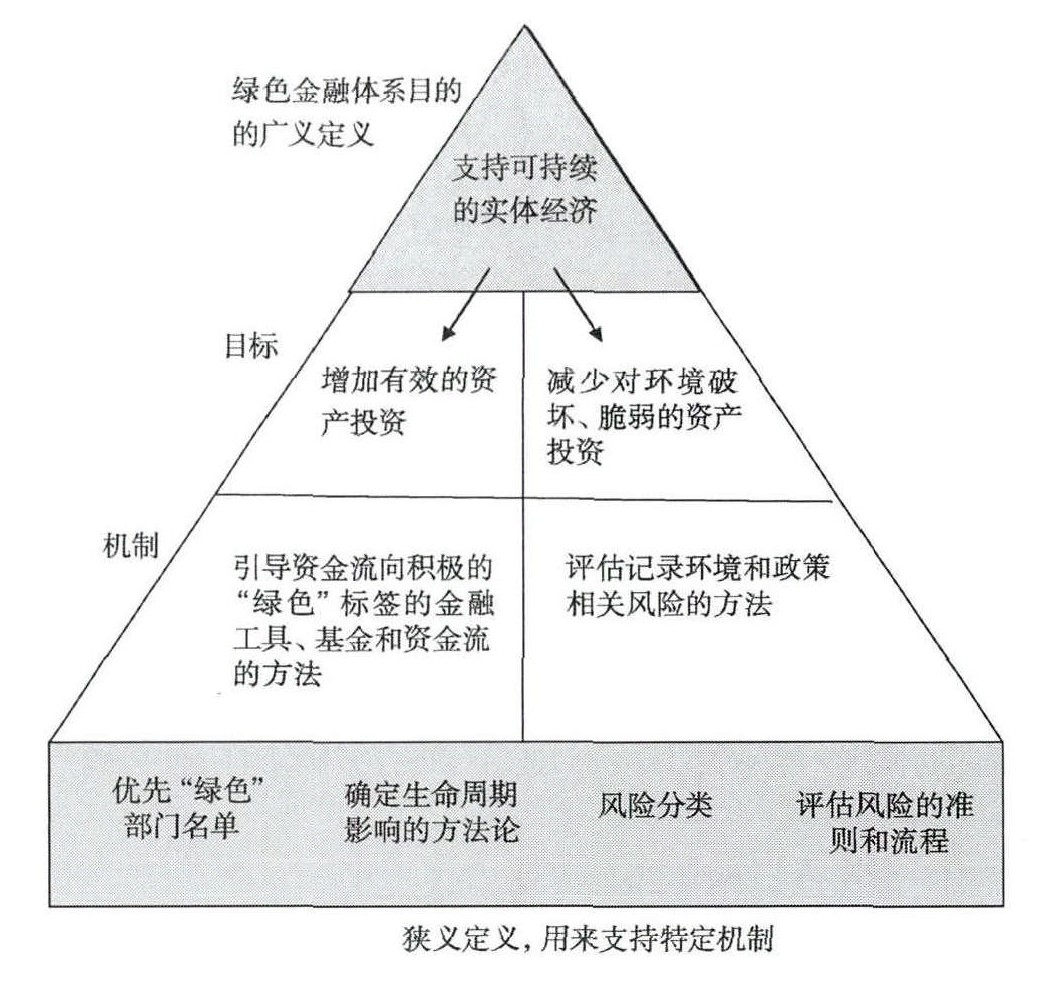
\includegraphics[width=0.5\linewidth]{./img/绿色金融定义.jpeg}
    \caption{绿色金融的定义。资料来源:联合国环境规划署}
\end{figure}

促进绿色金融的发展具有重要的战略意义。二十大报告中提出,“完善支持绿色发展的财税、金融、投资、价格政策和标准体系……推动形成绿色低碳的生产方式和生活方式”。无论是产业绿色升级、市场化要素配置,还是绿色消费,绿色金融都在其中起着关键作用。促进资源领域绿色金融的发展,有助于从资金、治理等方面为自然资源绿色高效开发利用提供保障\cite{王遥2016绿色金融对中国经济发展的贡献研究}。

\subsection*{绿色金融手段}
绿色金融工具主要在绿色金融市场中体现,绿色金融市场主要有绿色风投市场、绿色债券市场、绿色信贷市场、碳金融市场与绿色保险市场\cite{姚秋池2017国内外绿色金融研究综述}。

\citet{刘曼红2009绿色风险投资助推绿色}指出,面向绿色领域的风险投资“绿色风投”有助于提升GDP的同时减少自然资源消耗,减轻环境负载。

绿色债券则是为环境或气候相关收益的投资提供资金的一种固定收益证券,\citet{万志宏2016国际绿色债券市场}指出绿色债券促进资金向环境友好项目流动、契合了绿色经济与可持续发展理念。国际权威评级机构晨星对过去十年期间745份欧洲可持续投资基金样本进行了分析,发现绿色债券较传统投资基金的回报率更高,期间的收益波动更加平稳。

绿色信贷是我国最早也是目前我国最主流的绿色金融手段\cite{江红莉、王为东、王露、吴佳慧2020中国绿色金融发展的碳减排效果研究——以绿色信贷与绿色风投为例}。截至2021年末,国内21家主要银行绿色信贷余额达15.1万亿元,占其各项贷款的10.6\%。按照信贷资金占绿色项目总投资的比例测算,21家主要银行绿色信贷每年可支持节约标准煤超过4亿吨,减排二氧化碳当量超过7亿吨。\citet{陈柳钦2010国内外绿色信贷的实践路径}指出,绿色信贷指标指导银行机构在支持绿色产业发展、绿色低碳技术研发应用和传统行业节能改造的同时,对高碳行业实施重点、分类管理,遏制了高污染高排放项目盲目发展。

碳金融市场主要指碳排放权交易市场。\citet{肖序2007国际碳排放权交易市场研究}、\citet{李志学2014中国碳排放权交易市场运行状况}、\citet{刘明明2019论碳排放权交易市场失灵的国家干预机制}等指出碳金融市场的作用主要有:推动高排放行业实现产业结构和能源消费的绿色低碳化进而率先达峰、为碳减排释放价格信号并提供经济激励机制、为绿色低碳发展转型提供投融资渠道。

绿色保险市场以环境污染责任保险为代表,是在市场经济条件下进行环境风险管理的一项基本手段。\citet{严湘桃2009对构建我国}指出绿色保险在传统产业结构升级、构建绿色产业发展的过程中中发挥市场化风险管理作用。

\section*{共建“一带一路”国家目前环境现状}

\subsection*{部分共建“一带一路”国家生态环境脆弱}

一带一路国家幅员辽阔,国土面积接近世界的三分之一,但也承载了占世界人口总量70\%的人口,人口密度比世界平均水平高出近一倍,人地矛盾严重,人口与资源注定存在不匹配的矛盾。\citet{方恺2021}编制了环境可持续性赤字指数,指数越小,表示可持续性状况越好。当前“一带一路”地区的土地利用、碳排放、氮排放和磷排放均处于严重超载状态
\begin{figure}[H]
    \centering
    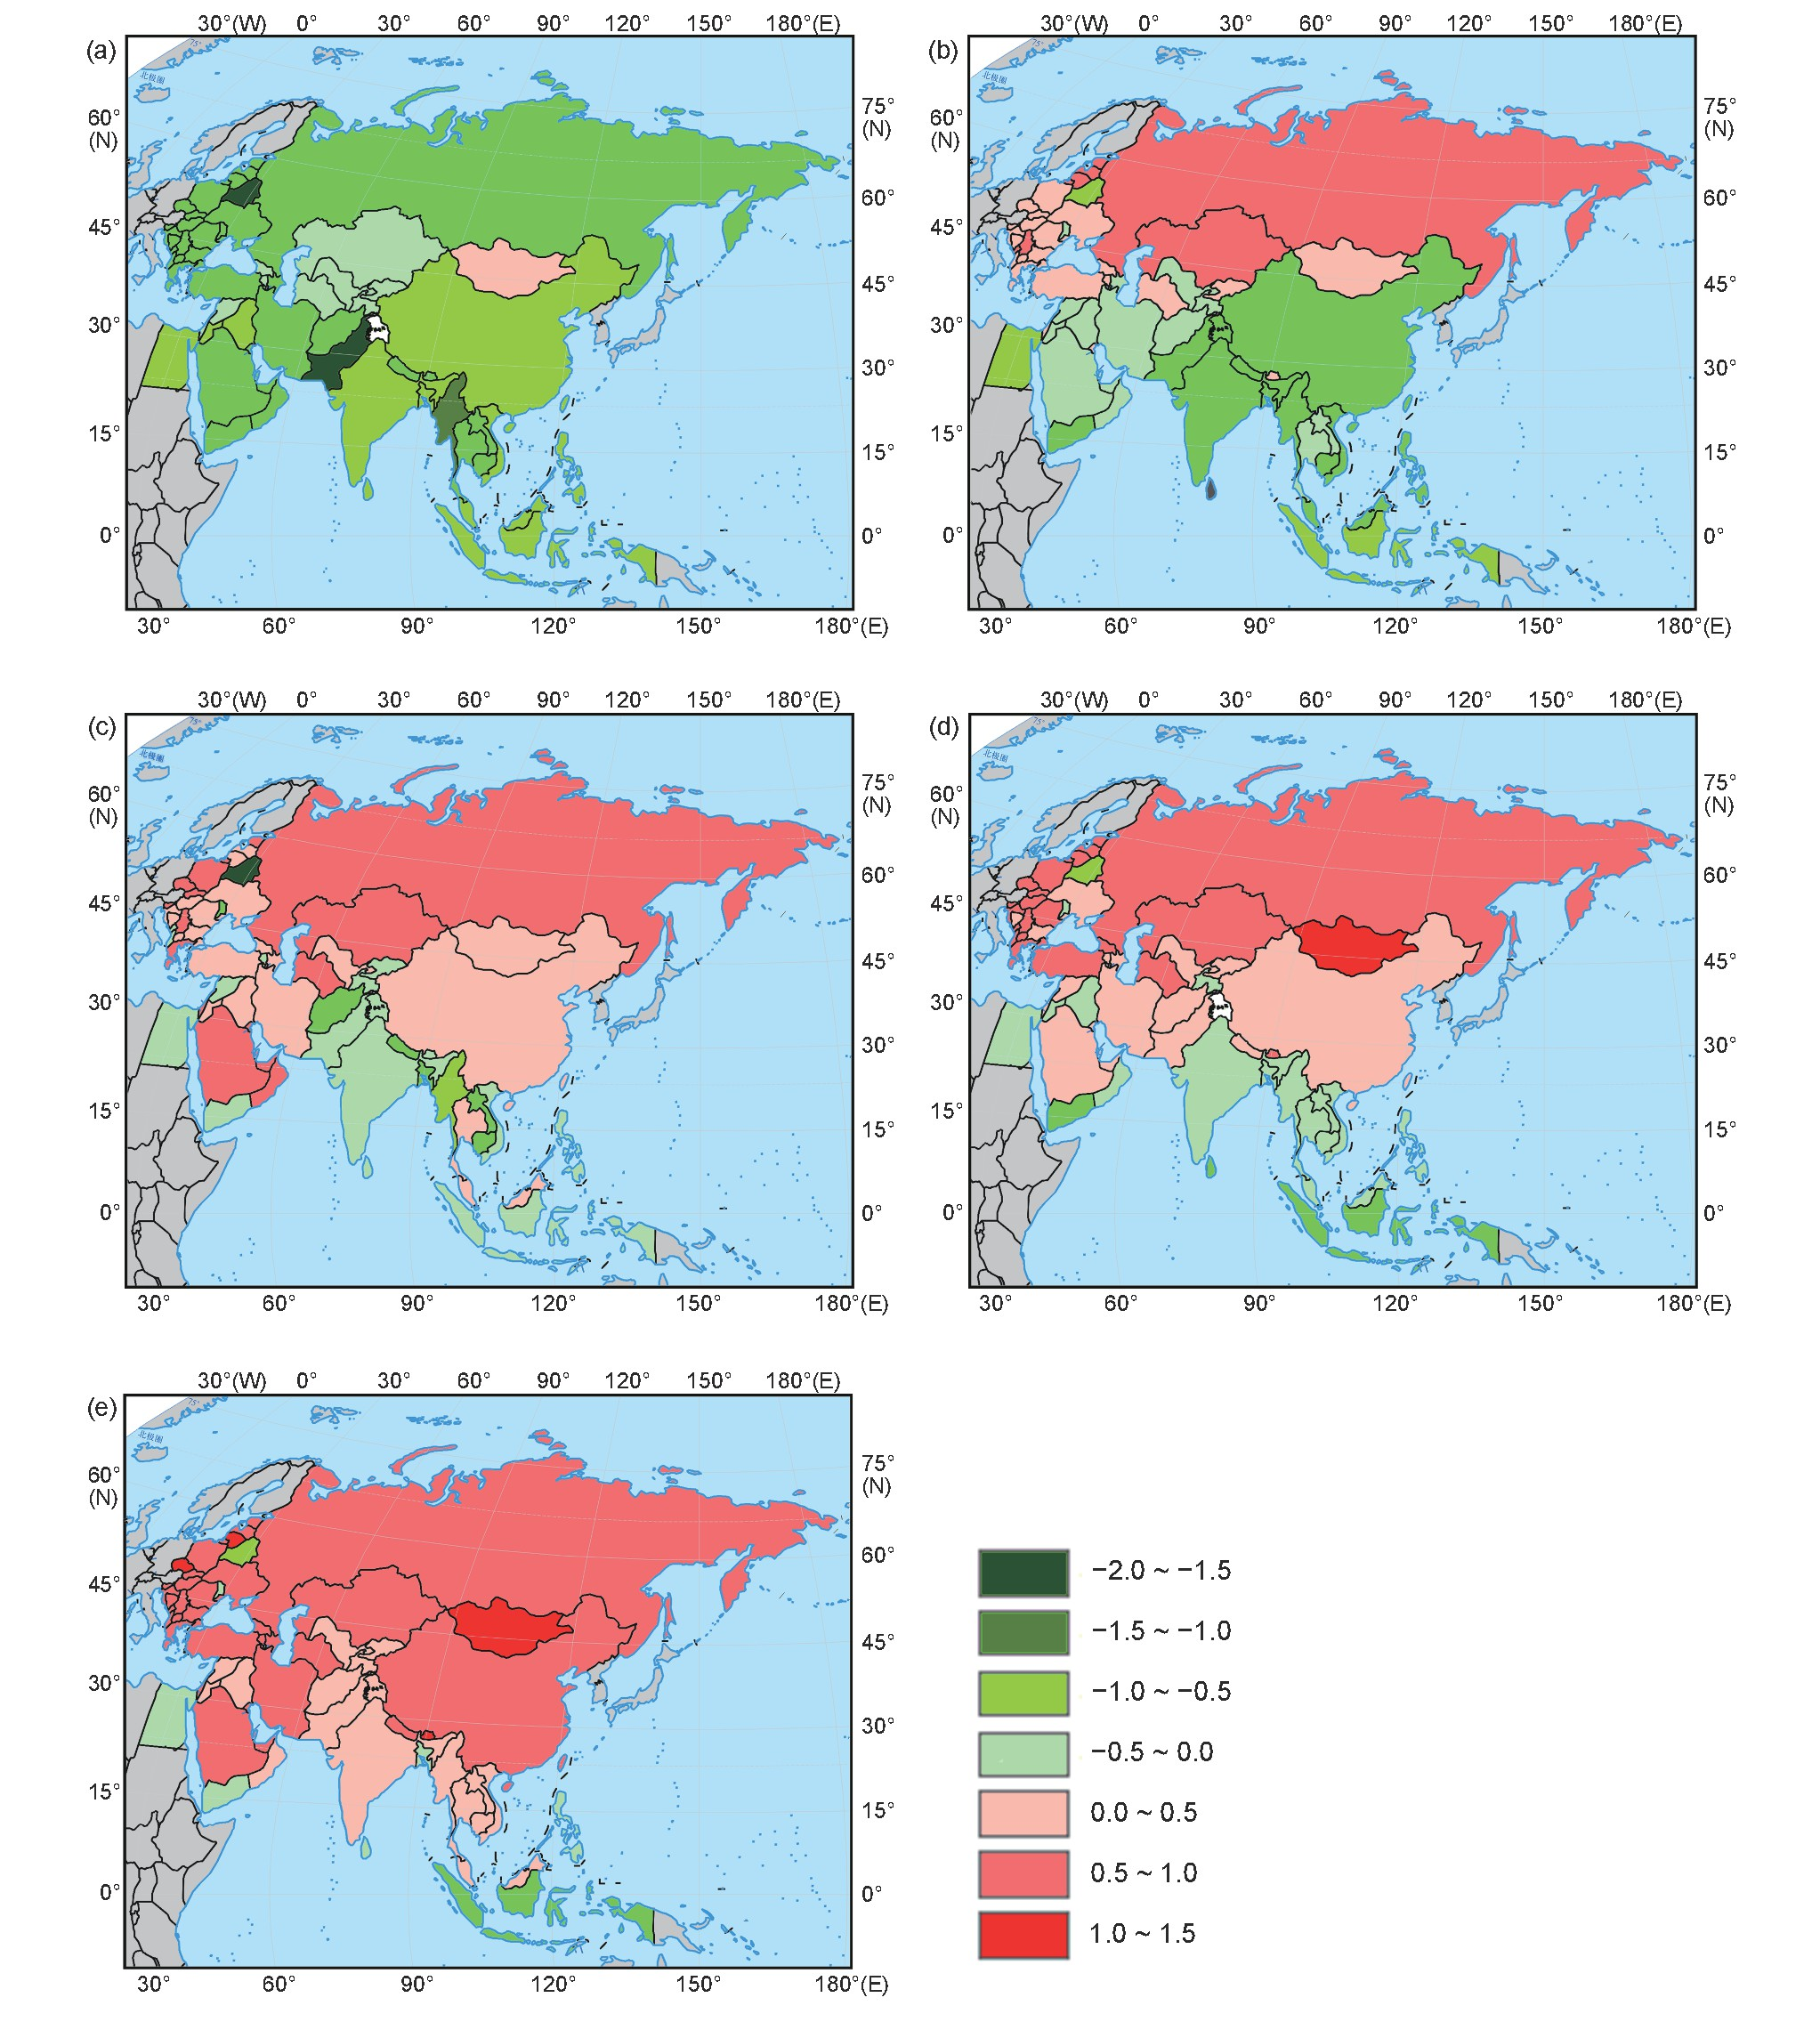
\includegraphics[width=0.8\linewidth]{img/ff.jpeg}
    \caption{水、土地、碳、氮和磷环境可持续性赤字指数\citet{方恺2021}}
\end{figure}

从区域看,沿线大部分国家和地区处于气候及地质变化的敏感地带,自然环境十分复杂,生态环境多样而脆弱。

东南亚尤其是东盟地区受热带季风影响,降水较多,洪水高发,也是世界生物最为多样最为丰富的地区之一,这一区域面临森林锐减、水和大气污染、工业污染排放、垃圾成灾、有毒化学品污染以及生物多样性锐减等问题。

中亚地区远离海洋,处于干旱和半干旱地区,是全球生态问题极为突出的地区,存在的环境问题主要有沙漠化和荒漠化严重、水资源短缺、水污染、大气污染等问题。同时,中亚地区处于欧亚板块交汇处,地震频繁,还面临生物多样性锐减、土壤污染以及重金属污染等环境问题。

南亚地区受每年的台风影响,洪水高发,水污染严重。印度遭受生活污水、工业排放废水、化学药品和固体废弃物的严重污染。

中东地区土壤贫瘠,处于干旱、半干旱地区,沙漠化和荒漠化问题严重,森林覆盖率低于世界平均水平。此外还遭受战争带来的“环境后遗症",还由于汽车和重工业发展,空气污染严重。

西亚面临土地荒漠化和森林进一步锐减问题,而蒙古和俄罗斯等国家由于人为过度放牧、无节制使用草地和矿产资源开发导致严重的草地荒漠化、沙尘暴和空气污染严重。

\subsection*{共建“一带一路”国家也采取了一定的环境管理措施}

共建“一带一路”国家普遍面临以上诸多环境问题,各国要求实现绿色发展、保护坏境的意愿在不断提高,绿色转型步伐在不断地加快,各国政府也在不断地采取措施加强环境保护相关的工作。由于共建“一带一路”国家面临的环境问题各不相同,各国采取的环境管理措施也各不相同。

从区域看,中亚国家比较重视绿色经济及生态安全,推动能源与环境相协调。哈萨克斯坦国情咨文中提出“绿色经济是哈萨克斯坦通往未来发展必经之路”。乌兹别克斯坦在“2013-2017年保护环境行动计划"中将环境可持续发展作为支柱行业,制定了“绿色经济原则的经济行业发展机制"。

东南亚各国忽视经济、社会和环境可持续发展的经济发展模式导致其发展受资源环境的约束越来越明显,资源过度开发和环境污染矛盾日益突出,要求各国必须加快推动绿色转型,实现可持续发展,明确绿色发展目标,推进绿色产业发展。马来西亚、缅甸、老挝、菲律宾和泰国等都将绿色发展纳入国家战略规划之中,并推进产业及相关政策变革。

南亚国家印度则提出要创建“绿色经济"大国,发展低碳经济。2008年国际金融危机爆发后,印度经济发展出现回落,国际能源价格动荡,不仅加重了印度能源负担,也严重影响了印度经济的长期发展。印度国内能源短缺特别是油气缺口巨大,成为制约其经济发展的瓶项,为降低能源短缺给本国经济发展造成的影响,印度极力发展低碳经济。

俄罗斯则倡导发展清洁能源,有效转变消费结构。长期以来,俄罗斯经济严重依赖石油、天然气出口,经济结构严重失衡,且不合理的资源开发给俄罗斯带来了较为严重的环境污染问题。随着世界能源环境的变化,俄罗斯经济出现低速增长甚至一度停滞,为减少传统能源型经济对环境的负面影响,促进经济稳定持续增长,俄罗斯开始注重向绿色经济转型,积极发展清洁能源技术,优化能源消费结构。
\section*{绿色金融潜在市场规模估测}
测算和厘清“一带一路”绿色投资需求的潜在规模可以更好地把握和理解“一带一路”国家绿色转型的困难,也有助于为“一带一路”国家绿色发展获得国际支持提供依据。

基于各国提交的自主贡献目标(NDC),我们采用自下而上方法估算未来10年“一带一路”国家绿色投资需求。具体的测算方法如下:

\begin{enumerate}
    \item 根据各国提交的NDC文件中制定的2030年具体行动计划,提取关键指标,包括但不限于:
          \begin{itemize}
              \item 减缓措施和适应措施的投入资金目标;
              \item 可再生能源目标装机量;
              \item 可再生能源发电量;
              \item 可再生能源发电量占比,这些指标是测算绿色投资规模的基础。
          \end{itemize}
    \item 将获得的数据进行分组:
          \begin{itemize}
              \item 一组是明确提出投入资金规模的66个国家,直接汇总其预期投资额为2.33万亿美元;
              \item 另一组是其他分别公布可再生能源具体规划的69个国家,据此测算其潜在的新能源投资2.8万亿美元
          \end{itemize}
    \item 最终汇总估计得出,2021-2030年间135个有效样本国家,按照GDP加权推算150个国家的绿色投资总需求将达到5.7万亿美元。
\end{enumerate}

未来10年5.7万亿美元、年均5700亿美元的绿色投资对这些国家而言压力很大,特别是在疫情冲击之后。从绝对规模上看,2019年这些国家固定资本形成总额约为3.8万亿美元。年均3600亿美元的资金需求约占其每年资本形成额的15\%,以每年新增15\%的投资推动绿色发展,对这些国家完成NDC的承诺构成了挑战。

与发达国家相比,“一带一路”国家绿色金融起步晚,且发展相对较慢,绿色金融作为空间巨大。“一带一路”代表性国家,如哈萨克斯坦于2020年首次发行绿色债券,由创业发展基金(Damu基金)在阿斯塔纳国际交易所注册并发行,规模为2亿坚戈(约300万人民币)、期限为36个月、票息率为11.75\%,募集资金将注入第二梯队银行和小额信贷组织,为中小企业在Damu基金绿色债券框架内开展的小型可再生能源投资项目提供更多融资。

\section*{促进“一带一路”绿色金融发展措施}
\subsection*{统一绿色标准,完善绿色金融基础设施}

“一带一路”国家多为发展中国家,金融体系本就不够发达,绿色金融基础设施建设更是相对滞后。各国在绿色标准、绿色评级、信息披露、统计监测和风险处置等方面存在空白或较大差异,这也是“一带一路”国家绿色金融发展相对较慢的原因。

以绿色金融标准为例,缺乏统一明确的标准定义可能导致绿色资金被用于非绿色项目,从而带来资金使用不当,非绿色项目的“洗绿”及跨国绿色投资风险问题。因此,促进绿色金融的发展,首先需要各国尽快建立与国际接轨的绿色统一标准,完善相关金融基础设施。

中国在助力“一带一路”国家完善绿色金融体系方面大有可为。截至目前,中国已就制订绿色投资原则、绿色金融能力建设等领域与共建“一带一路”国家开展了广泛的合作,例如人民银行在2018年指导发起的发起了《“一带一路”绿色投资原则》,已获得了包括来自巴基斯坦、哈萨克斯坦、蒙古等沿线国家的金融机构认可,中国与“一带一路”国家绿色金融合作空间广阔。

\subsection*{深化国际合作,发挥多边金融机构的支持作用}

多边金融机构对于大部分“一带一路”国家绿色金融发展而言有着重要的支持和引领作用。这其中包括:

\begin{enumerate}
    \item 多边金融机构可直接充当绿色资金的提供方,对“一带一路”国家提供必要的支持和帮助,尤其是投资期限长的大型项目。
    \item 多边金融机构参与对吸引私营部门投资发挥积极作用。多边金融机构投资的项目,在当地政策保险、贷款担保、优惠金融等方面易获得认可,比如,在所罗门群岛的蒂娜河水电开发项目中,绿色气候基金(GCF)提供了1,600万赠款以及40年内7,000万美元贷款的资金,从而使该项目可以满足私营部门投资者的回报期望,吸引私营部门投资进入。
    \item 多边金融机构可提供更多经验支持。大部分“一带一路”国家绿色产业在商业模式、金融工具、减排技术等领域处于探索和创新阶段,多边金融机构可提供更多经验支持,并为创新提供更多可能。
\end{enumerate}

\begin{table}[H]
    \centering
    \begin{tabular}{|c|c|c|}
        \hline
        名称          & 资金规模   & 出资方\\\hline
        气候投资基金(CIF) & 85亿美元  & 14个发达国家      \\
        绿色气候基金(GCF) & 178亿美元 & 24个会员国       \\
        适应基金(AF)    & 8亿美元   & 16个会员国       \\
        全球环境基金(GEF) & 200亿美元 & 184个会员国      \\\hline
    \end{tabular}
    \caption{著名的国际多边气候基金}
\end{table}

\subsection*{以公共部门投入带动私营部门投资者}

2017-2018年全球气候资金来源构成中,私营部门资金占比48\%,公共部门占比52\%,但是具体到“一带一路”国家而言,大部分绿色投资更多来源于政府和多边金融机构,私营部门投资者参与相对较少。推动绿色融资,公共部门也可以通过产品和机制创新调动私营部门参与“一带一路”绿色金融的积极性,包括公共资金担保、政府绿色采购等。

以肯尼亚LakeTurkana风电场项目为例,2014年非洲开发银行联合渣打银行向该项目提供了2千万欧元的担保,极大提振了私营部门投资者的信心,项目得以完成6.25亿欧元的筹资目标并于2018年顺利完工。

在私营部门投资者中,尤以机构投资者最为重要,包括养老基金、保险公司、对冲基金和共同基金。机构投资者的参与能够为绿色金融市场提供流动性,并为原来的债权方如商业银行打通退出渠道,进一步激活绿色投融资市场。然而,机构投资者投资于绿色金融产品的案例仍主要见于发达国家,例如瑞银在欧洲设立的全球最大绿色股权基金,而大部分发展中国家相对较少。未来,“一带一路”国家可考虑通过税收优惠、风险补偿、绩效评价等多方面给予优惠,尽可能吸引机构投资者参与绿色“一带一路”投资当中。

对于“一带一路”国家而言,实现绿色转型单纯依靠债权融资容易加重其还款付息压力,可能带来更高的债务风险。此外,考虑到这些国家的绿色转型刚刚起步,风险与机遇并存,其它诸如绿色股权、保险等金融工具更有利于促进国际间风险分担、提供长期资金。因此,“一带一路”绿色金融可借鉴国际先进经验,完善风险评估机制,丰富金融工具,以吸引更多形式的资金来源。

以中国为例,据美国企业研究所(AEI)的数据,中国对“一带一路”国家投资主要集中在能源和交通运输领域,特别地,2020年,中国对“一带一路”国家可再生能源投资占比达57\%,首次超过传统化石能源。随着“一带一路”国家绿色金融工具的不断发展和完善,预计中国股权类绿色投资规模有望进一步提升,从而更好地促进“一带一路”国家低碳转型发展。

\subsection*{将绿色发展理念嵌入更多金融合作进程}
以债务问题处置为例,2020年新冠疫情爆发后,对于发展中国家原本高企的对外债务压力更是雪上加霜,出现了普遍的流动性困难。2020年2月以来,共有40个国家和地区遭信用评级机构降级,已有6个国家相继违约。为应对这一局面,国际社会纷纷采取措施协助发展中国家渡过难关,包括债务暂缓偿付和G20债务处理共同框架。但国际社会要最终解决这一问题,仍需推出一套系统化的处置方案。

在解决“一带一路”发展中国家债务问题的过程当中,绿色金融同样可占据一席之地。一方面,债权方可在重组方案中采用债务气候转换、债务环境转换等工具,即要求债务国将部分减免额度再投资于气候、环境领域,还可允许债务国基于绿色项目发行绿色证券置换违约债务。通过赋予绿色属性,将债务处置与推动“一带一路”国家绿色转型相结合。另一方面,对于存量“一带一路”项目,可在甄别其绿色特征或绿色潜力基础上,基于项目现金流进行绿色资产证券化,或对国际投资者发行绿色债券,这也有助于推动存量项目的绿色转型。通过上述操作,本轮债务处置方案融入了绿色发展理念,更好与实现长期气候目标相契合。

\section*{结论}
绿色必将成为推进共建“一带一路”高质量发展更加鲜明的底色。当前共建“一带一路”国家面临着严峻的环境与发展问题,推进绿色发展是各国义不容辞的责任。2022年3月8日,经推进“一带一路”建设工作领导小组同意,国家发展改革委、外交部、生态环境部、商务部联合印发了《关于推进共建“一带一路”绿色发展的意见》,提出了进一步推进共建“一带一路”绿色发展,让绿色切实成为共建“一带一路”底色的总体要求,部署了绿色基础设施、绿色能源、绿色交通、绿色产业、绿色贸易、绿色金融、绿色科技、绿色标准和应对气候变化等绿色发展重点领域合作。

绿色金融潜在市场巨大,将推动一带一路高质量发展。在中国和越来越多共建“一带一路”国家和地区提出碳中和目标背景下,绿色金融在“一带一路”建设过程中从“锦上添花”变成“应有之义”。在此背景下,“一带一路‘建设将带来大量绿色投资机会,相关金融机构和投资者也要转变思路,从过去以防范环境和气候风险为主,转变为风险和机遇并重,抓住绿色投资和气候转型带来的重大发展机遇,绿色金融大有可为。
\nocite{*}
\printbibliography
\end{document}
